%!TEX root = ../thesis.tex

\section{背景}
近年,人手不足を背景にサービスロボットの需要が高まり,日常生活の中で目にする機会が増えている.現在,実用化に至っているサービスロボットは,館内の案内\cite{AYUDA:online},警備\cite{SQ-2:online},掃除\cite{KLEENBOT:online},配膳\cite{BellaBot:online},など,1つの作業に特化したロボットだが,複数作業が行える汎用サービスロボットであるモバイルマニピュレータロボットの開発が進められている.モバイルマニピュレータロボットは,自律移動ロボットにマニピュレータを搭載したロボットで,PAL Robotics社のTIAGo(図\ref{fig:TIAGo}参照) やトヨタ自動車のHSR(図\ref{fig:HSR}参照) などがある.これらのロボットは人に代わって様々な作業ができる汎用的なサービスロボットとして実用化が期待されている\cite{古賀達也201937_707}.本研究では,オフィス環境で活動するモバイルマニピュレータをオフィスロボットと定義して,話を進める.

オフィスロボットは様々な企業や研究室で開発が進められているが,設計データを公開しているものが少なく,標準的なプラットフォームが不足している.ロボットのオープンプラットフォームは,利用者によるハードウェアの改良などが容易にできるだけでなく,技術促進の場としても優れている.例えば,自律移動ロボットのオープンソースハードウェアであるi-Cartシリーズは,本研究室で開発されているorne-boxを始めとした様々なロボットのベースとして活用されている.ハードウェアプラットフォームがあると,ハードウェアを開発する手間が省け,ソフトウェア開発に注力できる.様々な開発者の知識や成果を共有し,技術の発展を加速させることに寄与すると考え,本研究ではオープンプラットフォームオフィスロボットの開発を行う.本項では,オフィスロボットのアームに着目し,設計と製作を行う.

\begin{figure}[h]
  \centering
  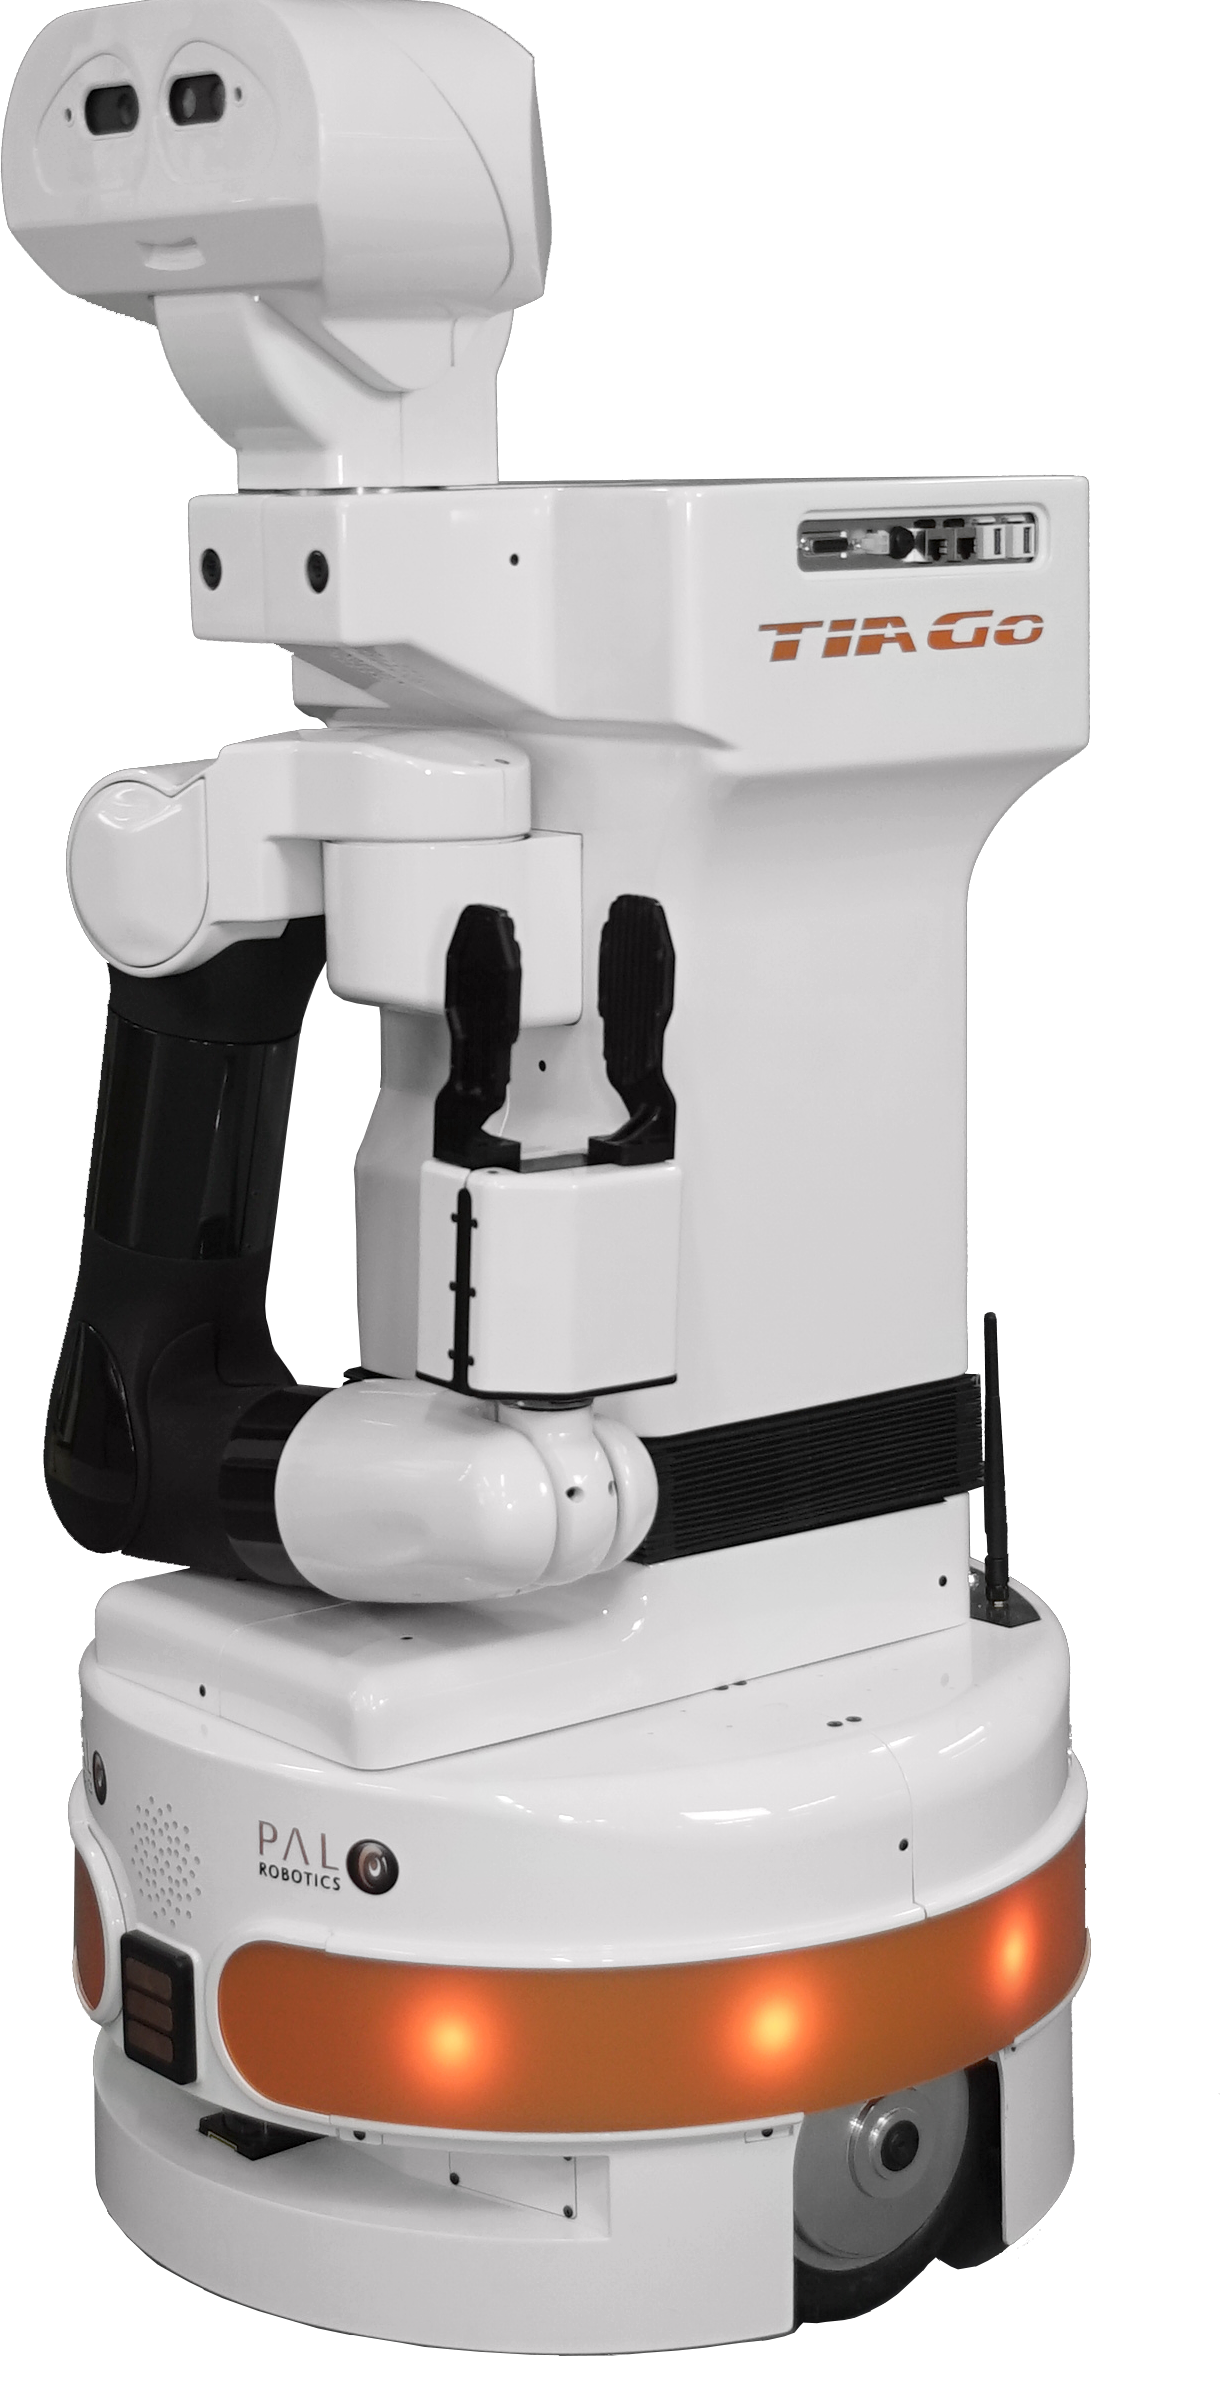
\includegraphics[width=25mm]{images/png/TIAGo.png}
  \caption{TIAGo from PAL-Robotics (source: \cite{TIAGo:online})}
  \label{fig:TIAGo}
\end{figure}
\begin{figure}[h]
  \centering
  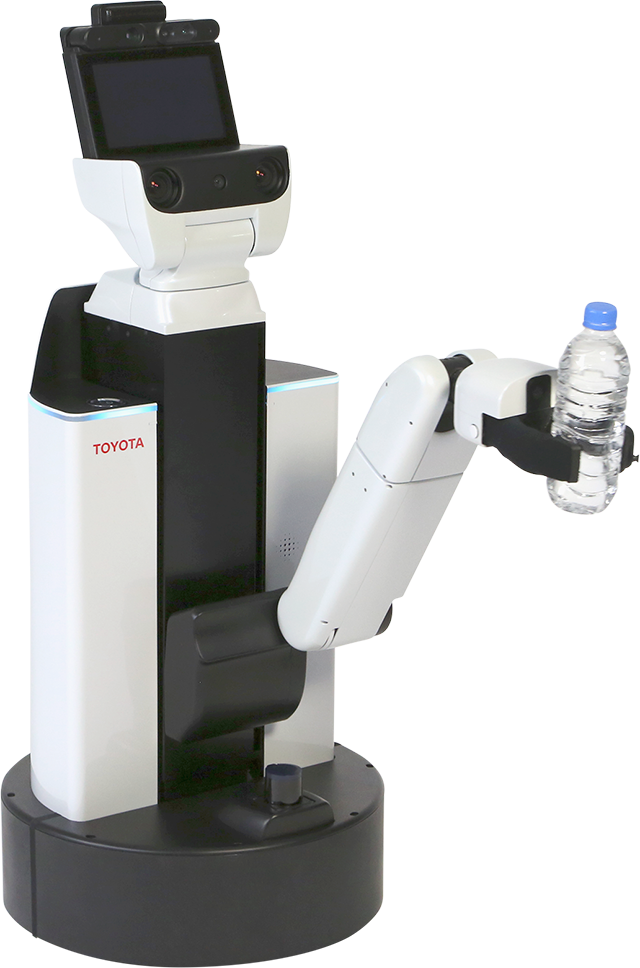
\includegraphics[width=25mm]{images/png/HSR.png}
  \caption{HSR from TOYOTA (source: \cite{HSR:online})}
  \label{fig:HSR}
\end{figure}

\newpage